\section{Tổng quan về công nghệ chuỗi khối}

\subsection{Công nghệ chuỗi khối}

\hspace{1cm}Công nghệ chuỗi khối là một cơ chế lưu trữ dữ liệu phân tán dựa
trên các khối thông tin được liên kết với nhau bằng phương thức mã hóa thông
tin. Các dữ liệu được lưu trên chuỗi có tính đồng bộ và nhất quán theo thời
gian. Hệ thống này dựa vào các giao thức đồng thuận để thay đổi thông tin bằng
cách thêm các khối mới vào trong chuỗi. Hiện tại có rất nhiều giao thức đồng
thuận đang được áp dụng từ việc tận dụng độ khó của các thuật toán mã hóa đến
đếm sự đồng thuận của các máy xác nhận trong hệ thống, tất cả đều tập trung vào
mục đích đảm bảo tính minh bạch và bất biến của các thông tin đang được lưu
trữ.

Bên cạnh đó, công nghệ chuỗi khối nhắm tới việc xây dựng một giao thức trao đổi
thông tin phi tập trung khi mà không có bất cứ một thực thể duy nhất nào có
quyền quyết định tới các thay đổi trong một chuỗi, cũng như dữ liệu sẽ được
phân phối về các nút trong mạng để đảm bảo yêu cầu về truy xuất và xác thực.
Bằng việc áp dụng công nghệ chuỗi khối, ta có thể giải quyết được vấn đề xác
thực giao dịch giữa những cá nhân hay tổ chức với nhau. Hiện tại, với các giao
dịch thông thường, chúng ta cần phải có một bên trung gian mà các bên tham gia
cùng tin cậy để làm chứng. Việc này có thể dẫn tới các rủi ro về bảo mật khi dữ
liệu của bên thứ ba bị thay đổi một cách không mong muốn. Hay tồi tệ hơn là
chính những bên trung gian xác thực này bắt tay với một vài cá nhân hay tổ chức
nhằm thao túng giao dịch, gây bất lợi cho các bên tham gia còn lại. Các lợi ích
chính của việc áp dụng công nghệ chuỗi khối có thể kể tới như cung cấp tính bảo
mật, giảm thiểu chi phí cho các giao dịch số. Bằng cơ chế phi tập trung và đồng
thuận thì việc giả mạo và thao túng các giao dịch này gần như là bất khả thi.
Có thể thấy rằng, công nghệ chuỗi khối trong thời gian gần đây đang được áp
dụng mạnh mẽ trong các giao dịch tài chính. Nhưng, sự áp dụng của công nghệ này
không chỉ dừng ở đó mà nó còn có thể được ứng dụng trong nhiều ngành nghề khác
như xác minh bản quyền, xác minh tính tin cậy nguồn gốc của sản phẩm, vv.

\subsection{Các mô hình chuỗi khối}

\hspace{1cm}Trong bối cảnh phát triển nhanh chóng của công nghệ chuỗi khối,
việc hiểu rõ về các mô hình chuỗi khối khác nhau là cần thiết để đánh giá và
lựa chọn giải pháp phù hợp cho các ứng dụng tài chính phi tập trung. Ba mô hình
chính của công nghệ chuỗi khối: công khai, riêng tư và liên hợp - mỗi mô hình
đều có
những đặc điểm, ưu điểm và hạn chế riêng, phản ánh sự đa dạng trong cách tiếp
cận với công nghệ sổ cái phân tán này.

Chuỗi khối công khai, như Bitcoin và Ethereum, là những mạng lưới mở và phi
tập trung hoàn toàn. Chúng cho phép bất kỳ ai cũng có thể tham gia vào quá
trình xác thực giao dịch và duy trì mạng lưới. Tính minh bạch và khả năng chống
can thiệp cao là những ưu điểm nổi bật của mô hình này. Tuy nhiên, chuỗi khối
công khai thường phải đối mặt với những thách thức về khả năng mở rộng và hiệu
suất, đặc biệt là khi số lượng giao dịch tăng cao. Cơ chế đồng thuận như Proof
of Work (PoW) trong Bitcoin, mặc dù đảm bảo an ninh mạng, nhưng lại tiêu tốn
nhiều năng lượng.

Ngược lại, chuỗi khối riêng tư được thiết kế để phục vụ cho nhu cầu cụ thể của
một tổ chức hoặc nhóm tổ chức. Trong mô hình này, quyền tham gia và xác thực
giao dịch được kiểm soát chặt chẽ. Hyperledger Fabric là một ví dụ điển hình
cho loại chuỗi khối này. Ưu điểm của chuỗi khối riêng tư là khả năng xử lý giao
dịch nhanh hơn và hiệu quả năng lượng cao hơn. Tuy nhiên, tính phi tập trung và
minh bạch - những đặc tính cốt lõi của công nghệ chuỗi khối - có thể bị giảm đi
trong mô
hình này.

Đứng giữa hai mô hình trên là mô hình chuỗi khối liên hợp, một giải pháp trung
gian kết
hợp ưu điểm của cả chuỗi khối công khai và riêng tư. Trong mô hình này, một
nhóm các tổ chức cùng quản lý mạng lưới, tạo ra một hệ thống bán tập trung. R3
Corda trong lĩnh vực tài chính là một ví dụ tiêu biểu. Chuỗi khối liên hợp cung
cấp một sự cân bằng giữa tính minh bạch và khả năng kiểm soát, đồng thời duy
trì hiệu suất cao hơn so với chuỗi khối công khai. Tuy nhiên, mô hình này cũng
đối mặt với thách thức trong việc điều phối giữa các thành viên và giải quyết
xung đột lợi ích.

Trong bối cảnh của dự án LaunchCrypt, sau khi cân nhắc kỹ lưỡng các mô hình
chuỗi khối hiện có, khóa luận quyết định lựa chọn mô hình chuỗi khối công khai
làm nền tảng cho hệ thống. Quyết định này dựa trên nhiều yếu tố quan trọng phù
hợp với mục tiêu và tầm nhìn của dự án. Thứ nhất, tính minh bạch và phi tập
trung của chuỗi khối công khai hoàn toàn phù hợp với tinh thần cốt lõi của tài
chính phi tập trung (DeFi), tạo ra một môi trường mở và công bằng cho tất cả
người dùng. Điều này đặc biệt quan trọng đối với LaunchCrypt, một nền tảng tập
trung vào việc tiếp cận với mọi người dùng. Thứ hai, khả năng chống can thiệp
và tính bất biến của dữ liệu trong chuỗi khối công khai sẽ đảm bảo tính toàn
vẹn của các giao dịch và thông tin token, tạo niềm tin cho người dùng - một yếu
tố then chốt trong việc xây dựng một hệ sinh thái tài chính mạnh mẽ. Cuối cùng,
việc chọn chuỗi khối công khai cũng phù hợp với mục tiêu hỗ trợ đa chuỗi của
LaunchCrypt, cho phép tích hợp dễ dàng với các chuỗi khối công khai lớn như
Avalanche, Solana và Aptos. Điều này mở rộng phạm vi tiếp cận của nền tảng và
tăng tính linh hoạt cho người dùng.

\subsection{Hợp đồng thông minh}

\hspace{1cm}Ethereum là một mạng phân tán được xây dựng dựa trên công nghệ
chuỗi khối bởi Vitalik Buterin vào năm 2014 với mục tiêu xây dựng các ứng dụng
phân quyền phi tập trung. Mạng Ethereum ngoài việc làm một cơ sở dữ liệu, nó
còn được sử dụng như một máy tính khổng lồ mà mọi người đều có thể truy cập
bằng cách lập trình và tương tác với các hợp đồng thông minh. Hợp đồng truyền
thống là tập hợp các điều khoản của một mối quan hệ và các ràng buộc này được
đảm bảo bởi sự đồng thuận của các bên tham gia và được bảo trợ bởi một bên
trung gian có quyền lực cao hơn (thường là các chính phủ). Còn hợp đồng thông
minh được đảm bảo bằng các đoạn mã, chúng có thể coi là các chương trình chạy
được trên chuỗi khối. Các giao dịch dựa trên hợp đồng thông minh bắt buộc phải
tuân thủ theo các điều khoản đã được lập trình sẵn để có thể được thực thi.
Cách thức hoạt động của hợp đồng thông minh là các đoạn mã sẽ được biên dịch và
ký bởi khóa của người tạo ra chúng, sau đó là triển khai trên chuỗi khối công
khai.
Một khi đã triển khai xong, bất cứ ai tham gia mạng lưới đều có thể sử dụng
chương
trình này và tạo ra các giao dịch nếu chúng phù hợp với các điều kiện đã đặt
ra. Tuy nhiên, các hợp đồng thông minh sẽ tồn tại bất biến cho nên nếu có bất
kỳ sai sót gì thì chỉ có thể tạo ra một hợp đồng mới thay cho cái cũ. Lợi ích
của việc sử dụng hợp đồng thông minh sẽ không yêu cầu xác minh danh tính của
các bên tham gia hay một bên trung gian đứng ra làm bên đại diện. Điều này giúp
tăng tốc độ và giảm chi phí giao dịch, cũng như xây dựng một môi trường giao
dịch không yêu cầu sự tin tưởng lẫn nhau. Ngoài ra, hợp đồng thông minh còn có
tính tùy chỉnh cao bởi vì chúng là những đoạn mã và có thể triển khai dễ dàng
bởi bất kỳ cá nhân nào tham gia mạng lưới, cung cấp đa dạng các cách thức và
giải pháp cho nhu cầu của người sử dụng.

Trong bối cảnh của dự án LaunchCrypt, hợp đồng thông minh đóng vai trò then
chốt
trong việc thực hiện mục tiêu phi tập trung quá trình tạo và giao dịch token.
LaunchCrypt sẽ triển khai một hệ thống hợp đồng thông minh đa chức năng trên
các
chuỗi khối công khai như Avalanche, Solana và Aptos, nhằm tự động hóa và đảm
bảo tính minh bạch cho toàn bộ quy trình. Đầu tiên, hợp đồng thông minh sẽ được
sử
dụng để tạo ra các token mới một cách dễ dàng và an toàn, cho phép người dùng
không có kiến thức chuyên sâu về lập trình vẫn có thể định nghĩa các tham số cơ
bản như tên token, ký hiệu và logo của token. Tiếp theo, LaunchCrypt sẽ triển
khai các hợp đồn thông minh quản lý thanh khoản, tự động tạo và duy trì các cặp
giao dịch cho các token mới, đảm bảo tính linh hoạt và hiệu quả trong quá trình
giao dịch. Cuối cùng, hợp đồng thông minh cũng được sử dùng để quản lý quá
trình
"tốt nghiệp" của token, tự động chuyển token lên các sàn giao dịch phi tập
trung lớn hơn khi đạt đủ điều kiện về thanh khoản và khối lượng giao dịch. Bằng
cách tận dụng tính bất biến và minh bạch của hợp đồng thông minh, LaunchCrypt
không
chỉ đảm bảo tính công bằng và an toàn cho người dùng, mà còn tạo ra một hệ sinh
thái tự động và hiệu quả, giúp tăng niềm tin của người dùng vào nền tảng.

\section{Tổng quan về tài chính phi tập trung (DeFi)}
\hspace{1cm}Là một dự án tập trung vào việc giải quyết các vấn đề trong lĩnh
vực tài chính phi tập trung, việc hiểu và nắm bắt được bản chất của tài chính
phi tập trung là điều vô cùng cần thiết và quan trọng. Nó không chỉ giúp định
hướng phương thức phát triển của LaunchCrypt mà còn đảm bảo rằng các giải pháp
được đề xuất sẽ phù hợp và hiệu quả trong bối cảnh DeFi đang không ngừng vươn
lên. Phần này sẽ làm rõ cách DeFi đang thay đổi cảnh quan tài chính truyền
thống, cũng như các cơ hội và thách thức mà nó mang lại. Đặc biệt, chúng ta sẽ
tập trung vào vai trò của DeFi trong việc tạo ra các thị trường tài chính mở,
minh bạch và không cần trung gian.

\subsection{Giới thiệu về tài chính phi tập trung}
\hspace{1cm}Tài chính phi tập trung (DeFi) đã nổi lên như một cuộc cách mạng
trong lĩnh vực tài chính, đánh dấu sự chuyển đổi từ hệ thống tài chính truyền
thống tập trung (CeFi) sang một mô hình mới, phi tập trung và mở. DeFi có thể
được định nghĩa là một hệ sinh thái các ứng dụng tài chính được xây dựng trên
nền tảng chuỗi khối, chủ yếu là Ethereum, nhằm tái tạo và mở rộng các dịch vụ
tài chính truyền thống mà không cần đến trung gian. Nguyên tắc cốt lõi của DeFi
bao gồm tính minh bạch, khả năng tương tác, và không cần sự tin cậy
(trustless), được thực hiện thông qua việc sử dụng các hợp đồng thông minh và
công
nghệ chuỗi khối. Điều này cho phép tạo ra các ứng dụng tài chính tự động, mở và
có thể kiểm chứng, từ đó giảm thiểu sự can thiệp của con người
và tăng cường tính công bằng trong hệ thống tài chính.

\subsection{Giới thiệu về sàn giao dịch phi tập trung (DEX)}
\hspace{1cm}Sàn giao dịch phi tập trung (Decentralized Exchanges - DEX) đã nổi
lên như một trong những ứng dụng quan trọng nhất của DeFi, cung cấp một phương
thức giao dịch tài sản kỹ thuật số mà không cần đến trung gian. Khác với sàn
giao dịch tập trung truyền thống, DEX hoạt động dựa trên hợp đồng thông minh
trên
các nền tảng chuỗi khối, cho phép người dùng duy trì quyền kiểm soát tài sản
của họ trong
suốt quá trình giao dịch. Cơ chế hoạt động cơ bản của DEX dựa trên việc kết nối
trực tiếp giữa người mua và người bán thông qua các giao thức được mã hóa, loại
bỏ nhu cầu về một bên trung gian đáng tin cậy. So với sàn giao dịch tập trung,
DEX mang lại nhiều ưu điểm đáng kể. Thứ nhất, DEX cung cấp tính minh bạch cao
hơn, với mọi giao dịch đều được ghi lại trên chuỗi khối công khai. Thứ hai,
người dùng duy trì quyền kiểm soát đối với khóa riêng tư, tức là quyền quyết
soát đối với chính tài sản của họ, từ đó giảm thiểu rủi ro mất mát
do hack hoặc lỗi của sàn giao dịch. Cuối cùng, DEX thường cung cấp danh sách
token đa dạng hơn, bao gồm cả các token mới và ít phổ biến. Tuy nhiên, DEX cũng
phải đối mặt với những thách thức như khả năng mở rộng hạn chế, chi phí gas cao
(đặc biệt trên mạng Ethereum), và trải nghiệm người dùng có thể phức tạp hơn
đối với người mới.

\section{Tổng quan về token và kiến trúc của token trên các chuỗi khối khác
  nhau}
\hspace{1cm}Để đề xuất giải pháp về việc tạo và giao dịch token trên
LaunchCrypt, việc hiểu rõ bản chất và cấu trúc của token trên các nền tảng
chuỗi khối khác nhau là điều cần phải nắm rõ. Phần này tập trung về việc nghiên
cứu các kiến thức nền tảng về token trên các chuỗi khối khác nhau, chỉ rõ cấu
trúc của các loại token, từ đó làm tiền đề khi triển khai module tạo token và
giao dịch trong suốt khóa luận.

\subsection{Tổng quan về token}
\hspace{1cm}Token trong bối cảnh công nghệ chuỗi khối là một dạng tài sản kỹ
thuật số
được tạo ra và quản lý trên một nền tảng chuỗi khối. Về bản chất, token là một
đại diện kỹ thuật số cho một quyền lợi hoặc giá trị cụ thể, có thể là tài sản,
tiện ích, hoặc quyền biểu quyết trong một hệ thống. Khác với cryptocurrency gốc
của một chuỗi (như Bitcoin trên mạng Bitcoin hoặc Ether trên Ethereum),
token thường được tạo ra và quản lý thông qua hợp đồng thông minh trên một
chuỗi khối hiện có. Các đặc điểm cơ bản của token bao gồm khả năng chuyển
nhượng, tính chia nhỏ, giá trị đại diện, và tính xác thực. Token có thể được
chuyển từ một địa chỉ này sang địa chỉ khác một cách dễ dàng và nhanh chóng.
Nhiều loại token có thể được chia thành các đơn vị nhỏ hơn, cho phép giao dịch
với số lượng linh hoạt. Mỗi token đại diện cho một giá trị cụ thể trong hệ
thống mà nó hoạt động, và mọi giao dịch liên quan đến token đều được xác thực
và ghi lại trên chuỗi khối, đảm bảo tính minh bạch và an toàn.

\subsection{Kiến trúc token trên Ethereum}
\hspace{1cm}ERC-20 (Ethereum Request for Comment 20) \cite{ERC20} là tiêu chuẩn
token phổ biến nhất trên chuỗi khối Ethereum. ERC-20 đã trở thành nền tảng cho
hầu hết các fungible token trên Ethereum. Tiêu chuẩn này định nghĩa một tập hợp
các quy tắc mà một token trên Ethereum phải tuân theo, đảm bảo tính tương thích
và nhất quán trong hệ sinh thái Ethereum. ERC-20 định nghĩa một interface bao
gồm 9 hàm bắt buộc và 2 sự kiện. Cấu trúc cơ bản như sau:

\begin{center}
    \begin{tabular}{c p{0.9\textwidth}}
        \hline
        \multicolumn{2}{l}{\textbf{ERC20:} \textit{Fungible token standard
                function
                in Ethereum}}
        \\ \hline
        1 & \hspace{1em} function \textbf{name}() public view returns (string)
        \\
        2 & \hspace{1em} function \textbf{symbol}() public view returns
        (string)
        \\
        3 & \hspace{1em} function \textbf{decimals}() public view returns
        (uint8)
        \\
        4 & \hspace{1em} function \textbf{totalSupply}() public view returns
        (uint256)
        \\
        5 & \hspace{1em} function \textbf{balanceOf}(address \textbf{owner})
        public view returns                                                    \\
          & \hspace{1em}(uint256 \textbf{balance})                             \\
        6 & \hspace{1em} function \textbf{transfer}(address \textbf{to},
        uint256
        \textbf{value}) public returns                                         \\
          & \hspace{1em} (bool \textbf{success})                               \\
        7 & \hspace{1em} function \textbf{transferFrom}(address \textbf{from},
        address \textbf{to}, uint256 \textbf{value})
        \\  & \hspace{1em}public returns (bool
           \textbf{success})
        \\
        8 & \hspace{1em} function \textbf{approve}(address \textbf{spender},
        uint256 \textbf{value}) public returns
        \\
          & \hspace{1em} (bool \textbf{success})                               \\
        9 & \hspace{1em} function \textbf{allowance}(address \textbf{owner},
        address \textbf{spender}) public view                                  \\
          & \hspace{1em}returns (uint256 \textbf{remaining})                   \\
        \hline
    \end{tabular}
\end{center}



\begin{center}
    \begin{tabular}{c p{0.9\textwidth}}
        \hline
        \multicolumn{2}{l}{\textbf{ERC20:} \textit{Fungible token standard
                event in
                Ethereum}}
        \\ \hline
        1 & \hspace{1em} event \textbf{Transfer}(address indexed \textbf{from},
        address indexed \textbf{to}, uint256 \textbf{value})
        \\
        2 & \hspace{1em} event \textbf{Approval}(address indexed
        \textbf{owner},
        address indexed \textbf{spender}, uint256 \textbf{value})
        \\
        \hline
    \end{tabular}
\end{center}

\hspace{-1cm}Mỗi hàm và sự kiện trong cấu trúc này có một vai trò cụ thể:
\begin{itemize}
    \item \textbf{name}: Trả về tên của token được hiển thị trên chuỗi (Ví
          dụ: Ethers).

    \item \textbf{symbol}: Trả về ký hiệu rút gọn của token được hiển thị trên
          chuỗi (Ví dụ: ETH).

    \item \textbf{decimals}: Trả về số chữ số thập phân được sử dụng để biểu
          diễn một đơn vị nhỏ nhất của token (Ví dụ: 18).

    \item \textbf{totalSupply}: Trả về tổng cung hiện tại của token trên toàn
          bộ chuỗi.

    \item \textbf{balanceOf}: Trả về số dư token của một địa chỉ cụ thể.

    \item \textbf{transfer}: Thực hiện chuyển một số lượng token từ địa chỉ
          người gửi đến một địa chỉ khác.

    \item \textbf{transferFrom}: Thực hiện chuyển token từ một địa chỉ này sang
          địa chỉ khác, sử dụng cơ chế allowance.

    \item \textbf{allowance}: Kiểm tra số lượng token mà một địa chỉ được phép
          chi tiêu thay cho chủ sở hữu.

    \item \textbf{approve}: Cho phép một địa chỉ chi tiêu một số lượng token
          thay mặt chủ sở hữu.
\end{itemize}

\hspace{-1cm}Sự kiện \textbf{Transfer} và \textbf{Approval} được phát ra khi có
sự chuyển token hoặc phê duyệt chi tiêu, giúp các ứng dụng bên ngoài theo dõi
hoạt động của token.

\hspace{-1cm}Ngoài ra, để kiểm soát nguồn cung và kiểm soát lạm phát, các token
tuân theo tiêu chuẩn ERC20 thường xây dựng các hàm nội bộ sau:

\begin{center}
    \begin{tabular}{c p{0.9\textwidth}}
        \hline
        \multicolumn{2}{l}{\textbf{ERC20:} \textit{Fungible token standard
                internal
                function in Ethereum}}
        \\ \hline
        1 & \hspace{1em} function \textbf{mint}(address \textbf{account},
        uint256
        \textbf{value}) internal
        \\
        2 & \hspace{1em} function \textbf{burn}(address \textbf{account},
        uint256
        \textbf{value}) internal
        \\
        \hline
    \end{tabular}
\end{center}

\hspace{-1cm}Trong đó, hàm \textbf{mint} thường được sử dụng để đúc 1 lượng
token ban đầu cho người khởi tạo token, \textbf{burn} là hàm được sử dụng để
"đốt" một lượng token ở một địa chỉ cụ thể, giúp hạn chế lạm phát và điều chỉnh
tổng cung của token theo xu hướng giảm đi.

\subsection{Kiến trúc token trên Solana}
\hspace{1cm}Solana, một chuỗi khối hiệu suất cao, có cách tiếp cận khác biệt so
với Ethereum trong việc triển khai và quản lý token. Thay vì sử dụng smart
contracts như Ethereum, Solana sử dụng một chương trình có sẵn gọi là Token
Program để quản lý việc tạo và giao dịch token. Phần này sẽ đề cập đến những
kiến thức cơ bản về cách token được triển khai trên Solana. Chúng được gọi là
SPL (Solana program library) ~\cite{SPL}. Dưới đây là 3 thành phần cơ bản giúp
cho token hoạt động được trên Solana.

\begin{itemize}
    \item \textbf{Token Program}: Chứa tất cả logic để tương tác với các token
          trên Solana (kể cả fungible và non-fungible token).

    \item \textbf{Mint Account}: Đại diện cho một loại token cụ thể và lưu trữ
          metadata toàn cầu về token, chẳng hạn như tổng nguồn cung và quyền
          đúc (địa chỉ
          được ủy quyền để tạo token mới).

    \item \textbf{Token Account}: Tài khoản đại diện cho sự sở hữu 1 loại token
          ứng với 1 user.
\end{itemize}
Token Program chứa một số chức năng chính, bao gồm:
\begin{itemize}
    \item \textbf{InitializeMint}: Tạo ra 1 \textbf{Mint Account} để đại diện
          cho một token mới trên Solana

    \item \textbf{InitializeAccount}: Tạo ra 1 \textbf{Token Account} mới.

    \item \textbf{MintTo}: Tạo ra một lượng mới của một loại token cụ thể và
          thêm chúng vào một token account. Điều này làm tăng nguồn cung token
          và chỉ có
          thể được thực hiện bởi địa chỉ có thẩm quyền.

    \item \textbf{Transfer}: Chuyển một lượng token từ token account này sang
          token account khác.

\end{itemize}
Token trên Solana được xác định duy nhất bằng địa chỉ của Mint Account do Token
Program sở hữu. Tài khoản này là một bộ đếm toàn cầu cho một loại token cụ thể
và lưu trữ dữ liệu như:

\begin{itemize}
    \item \textbf{Supply}: Tổng lượng cung hiện tại của token.

    \item \textbf{Decimals}: Số chữ số thập phân được sử dụng để biểu diễn một
          đơn vị nhỏ nhất của token.

    \item \textbf{Mint authority}: Địa chỉ được cấp quyền cho việc tạo ra token
          mới, điều này làm tăng tổng cung của token.

    \item \textbf{Freeze authority}: Địa chỉ được cấp quyền cho việc đóng băng
          token (dừng các hoạt động chuyển token qua lại giữa các token
          account).

\end{itemize}
Sau đây là thông tin lưu trữ của Mint Account được triển khai trong Solana:

\begin{center}
    \begin{tabular}{c p{0.9\textwidth}}
        \hline
        \multicolumn{2}{l}{\textbf{Solana Mint Account} }
        \\  \hline
        1 & \textbf{pub} struct \textbf{Mint} \textbraceleft
        \\
        2 & \hspace{1em} \textbf{pub} mint\textunderscore authority:
        COption<\textbf{Pubkey}>
        \\
        3 & \hspace{1em} \textbf{pub} supply: \textbf{u64}
        \\
        4 & \hspace{1em} \textbf{pub} decimals: \textbf{u8}
        \\
        5 & \hspace{1em} \textbf{pub} is\textunderscore initialized:
        \textbf{bool}
        \\
        6 & \hspace{1em} \textbf{pub} freeze\textunderscore authority:
        COption<\textbf{Pubkey}>
        \\
        7 & \textbraceright
        \\

        \hline
    \end{tabular}
\end{center}
\begin{figure}[h!]
    \begin{center}
        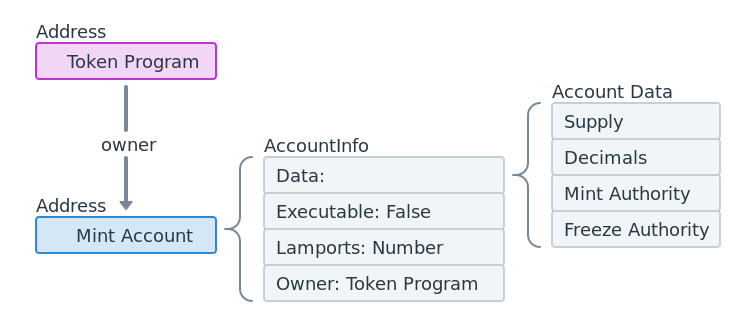
\includegraphics[width=0.85\textwidth]{figures/c1/mint-account.png}
        \caption{Cấu trúc của Mint Account trên solana.~\cite{SPL}}
        \label{fig:feature_interaction_example}
    \end{center}
\end{figure}
Để theo dõi quyền sở hữu riêng lẻ của từng đơn vị token cụ thể, Token Program
phải tạo ra một loại tài khoản dữ liệu khác. Trong cấu trúc token của Solana,
loại tài khoản này được gọi là Token Account.
Dữ liệu được lưu trữ trên Token Account bao gồm:
\begin{itemize}
    \item \textbf{Mint}: Loại token mà Token Account này đang nắm giữ.

    \item \textbf{Owner}: Tài khoản được ủy quyền để thực hiện các giao dịch
          trên Token Account.

    \item \textbf{Amount}: Số lượng token mà Token Account này đang nắm giữ.
\end{itemize}

\hspace{-1cm}Để một ví sở hữu đơn vị của một token nhất định, nó cần tạo một
Token Account cho loại Token (Mint Account) tương ứng và chỉ định ví đó là chủ
sở hữu của Token Account. Một ví có thể tạo nhiều Token Account cho cùng một
loại token, nhưng mỗi Token Account chỉ có thể được sở hữu bởi một ví và nắm
giữ các đơn vị của một loại token.

\begin{figure}[h!]
    \begin{center}

        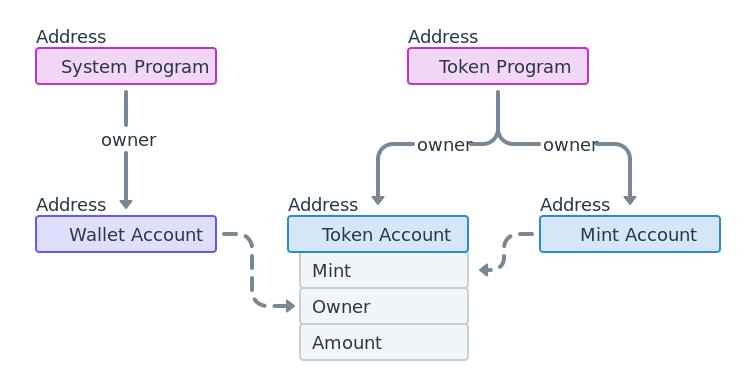
\includegraphics[width=0.85\textwidth]{figures/c1/token-account-relationship.png}
        \caption{Account relationship trên solana.~\cite{SPL}}
        \label{fig:feature_interaction_example}
    \end{center}
\end{figure}
\hspace{-1cm}Tuy nhiên, để đơn giản hóa quá trình định vị địa chỉ Token Account
cho một owner và một Mint Account cụ thể, Solana đã đưa ra giải pháp sử dụng
Associated Token Accounts.

\hspace{-1cm}Associated Token Accounts là Token Account có địa chỉ được xác
định rõ ràng bằng cách sử dụng địa chỉ của owner và địa chỉ của Mint Account.
Có thể coi rằng Associated Token Accounts là Token Account "mặc định" cho một
owner và một Mint Account cụ thể. Điều quan trọng phải hiểu rằng Associated
Token Accounts không phải là một Token Account khác, đó chỉ là một loại Token
Account có địa chỉ cụ thể được xác định từ trước.

\begin{figure}[h!]
    \begin{center}

        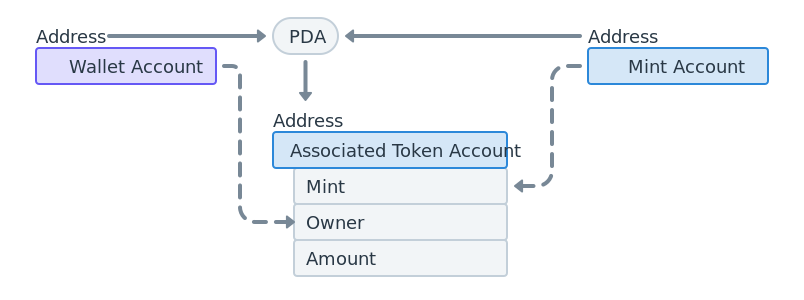
\includegraphics[width=0.85\textwidth]{figures/c1/associated-token-account.png}
        \caption{Associated Token Account trên solana.~\cite{SPL}}
        \label{fig:feature_interaction_example}
    \end{center}
\end{figure}

\hspace{-1cm}Cuối cùng, ta có quan hệ giữa Wallet account, Associated Token
Account và mint account như sau:

\begin{figure}[h!]
    \begin{center}

        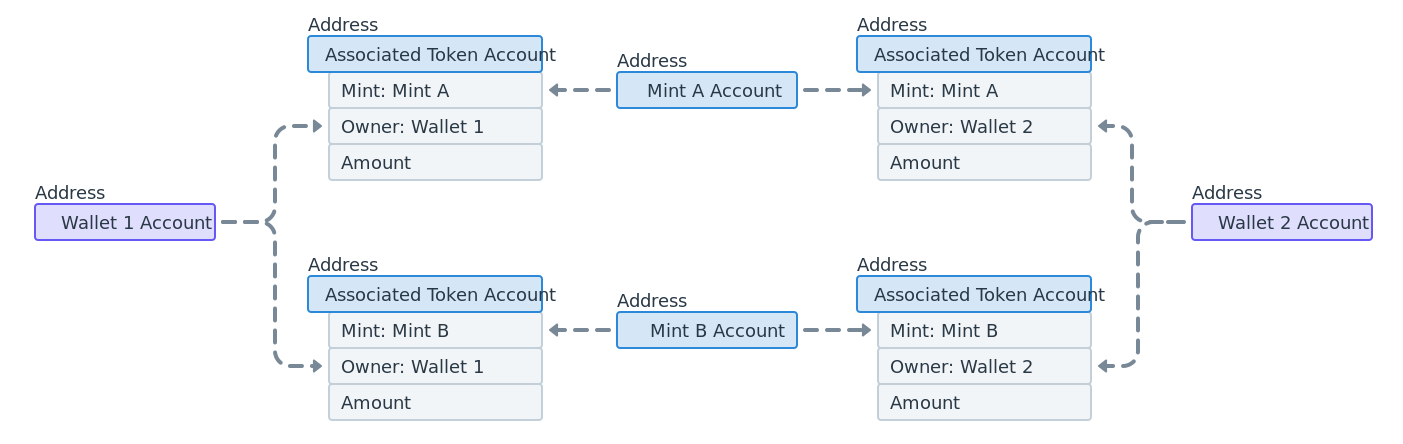
\includegraphics[width=1\textwidth]{figures/c1/token-account-relationship-ata.png}
        \caption{Quan hệ giữa các loại tài khoản trên solana.~\cite{SPL}}
        \label{fig:feature_interaction_example}
    \end{center}
\end{figure}

\subsection{Kiến trúc token trên Aptos}
Tiêu chuẩn token trên Aptos ~\cite{FA} (còn được gọi là “\textbf{Fungible
    Asset}” hoặc "\textbf{FA}") cung cấp một cách tiêu chuẩn, an toàn về type
để
xác định token trong hệ sinh thái Move. Tiêu chuẩn này cho phép chuyển và tùy
chỉnh các token cho mọi trường hợp sử dụng. Trong Aptos, với tiêu chuẩn
“\textbf{Fungible Asset}”, token được biểu diễn dưới dạng một object chứa data.
Tiêu chuẩn này cung cấp các chức năng như tạo, đúc, chuyển và đốt (burn) các
token. Để thực hiện điều này, tiêu chuẩn “\textbf{Fungible Asset}” sử dụng hai
Move object như sau:
\begin{itemize}
    \item \textbf{Object<Metadata>}: Đối tượng này thể hiện thông tin chi tiết
          về chính Fungible Asset, bao gồm thông tin như name, symbol và
          decimals.

    \item \textbf{Object<Fungible Store>}: Đối tượng này lưu trữ số lượng đơn
          vị Fungible Asset được sở hữu bởi tài khoản tương ứng. Fungible Asset
          có thể
          hoán đổi với bất kỳ Fungible Asset có cùng siêu dữ liệu (metadata).
          Một tài
          khoản có thể sở hữu nhiều FungibleStore cho một Fungible Asset duy
          nhất, nhưng
          điều này chỉ áp dụng cho các trường hợp sử dụng nâng cao.

\end{itemize}
Sơ đồ bên dưới thể hiện mối quan hệ giữa các object này. Đối tượng
\textbf{metadata} được sở hữu bởi người tạo \textbf{FA}, sau đó được tham chiếu
trong \textbf{FungibleStores} của chủ sở hữu \textbf{FA} để cho biết
\textbf{FA} nào đang được theo dõi:

\begin{figure}[H]
    \begin{center}
        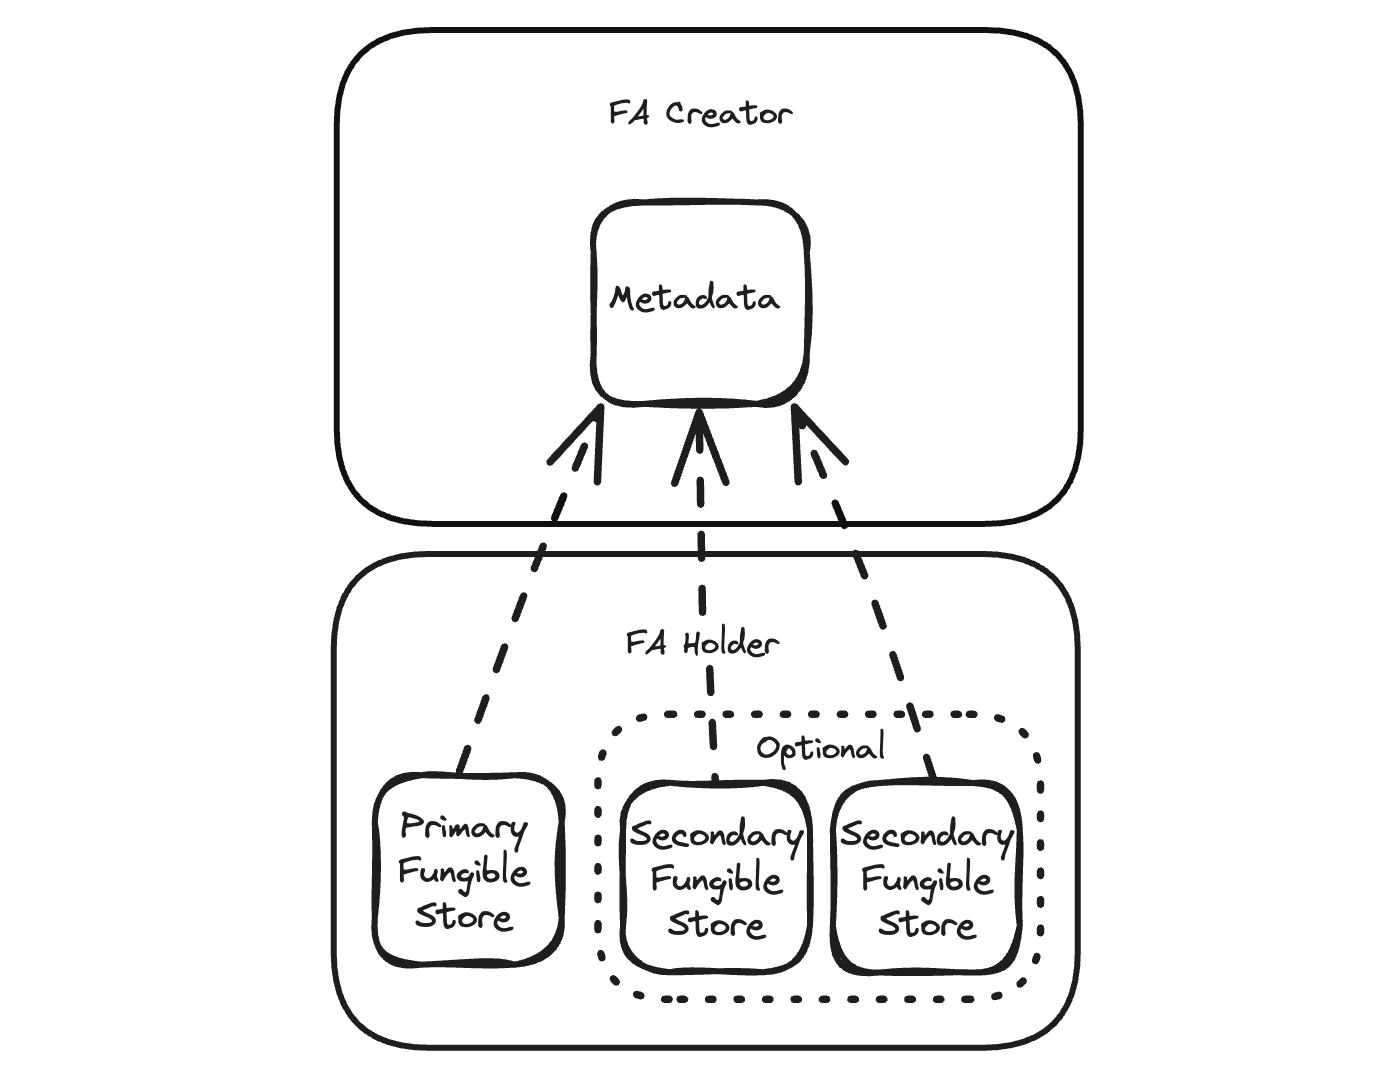
\includegraphics[width=1\textwidth]{figures/c1/fa-diagram-light.png}
        \caption{Mối quan hệ giữa Metadata và Fungible Store trong Aptos.~\cite{FA}}
        \label{fig:feature_interaction_example}
    \end{center}
\end{figure}
\hspace{-1cm}Như vậy, khi người dùng muốn chuyển \textbf{Fungible Asset} từ địa
chỉ này sang địa chỉ khác, về bản chất, Aptos sẽ cập nhật lại thông tin về số
lượng \textbf{Fungible Asset} còn lại trong các \textbf{Fungible Store} ứng với
mỗi người dùng. Về các chức năng còn lại của token, Aptos cung cấp các
\textbf{reference} (ref) được tạo ngay khi \textbf{Fungible Asset} được tạo ra.
Một số ref phổ biến được sử dụng trong tiêu chuẩn \textbf{Fungible Asset} như
sau:

\begin{itemize}
    \item \textbf{ConstructorRef}: Tham chiếu cho phép FA được tùy chỉnh ngay
          sau khi chúng được tạo ra. Thông thường, constructorRef được sử dụng
          để tạo ra
          các ref khác.

    \item \textbf{MintRef}: Cung cấp khả năng tạo ra các đơn vị FA mới.

    \item \textbf{TransferRef}: Cung cấp khả năng đóng băng các tài khoản khỏi
          việc chuyển FA hoặc bỏ qua việc đóng băng hiện có. (Điều này có thể
          quan trọng
          khi cố gắng tuân thủ một số quy định).

    \item \textbf{BurnRef}: Cung cấp khả năng xóa các đơn vị FA.
\end{itemize}
\textit{Lưu ý}: Tất cả các tham chiếu phải được tạo khi đối tượng được tạo vì
đó là lần duy nhất có thể tạo ConstructorRef của đối tượng.

\section{Automated Market Maker (AMM)}
\hspace{1cm}Một trong những đổi mới quan trọng nhất trong lĩnh vực DEX là sự ra
đời của Automated Market Maker (AMM). AMM là một loại DEX đặc biệt sử dụng các
thuật toán để tự động định giá và cung cấp thanh khoản cho các cặp giao dịch.
Thay vì dựa vào sổ lệnh truyền thống (Order book), AMM sử dụng các pool thanh
khoản, nơi người dùng có thể đóng góp tài sản và nhận lại token thanh khoản đại
diện cho phần đóng góp của họ. Công thức phổ biến nhất cho AMM là \textbf{X*Y=K
    (1)}, trong đó X và Y là số lượng của hai tài sản trong pool, và k là một
hằng
số.

\subsection{Công thức trao đổi token trên AMM}
\hspace{1cm}Khi một giao dịch xảy ra, số lượng còn lại của 2 token ( từ nay gọi
là \textbf{tokenA} và \textbf{tokenB}) trong pool sẽ thay đổi. Tuy nhiên, tích
số lượng còn lại của 2 token trong pool sẽ không đổi, luôn luôn bằng k. Bây
giờ, chúng ta cùng xét một ví dụ, giả sử ta sẽ bán một lượng tokenA để nhận lại
1 lượng tokenB. Ta có:
\[
    dX = \text{Số lượng } {\text{tokenA}} \text{ bán}
\]
\[
    dY = \text{Số lượng } {\text{tokenB}} \text{ nhận}
\]
Sau quá trình này, theo công thức X*Y=K, ta có:
\[
    (X+dX)(Y-dY) = K
\]

\begin{figure}[H]
    \begin{center}
        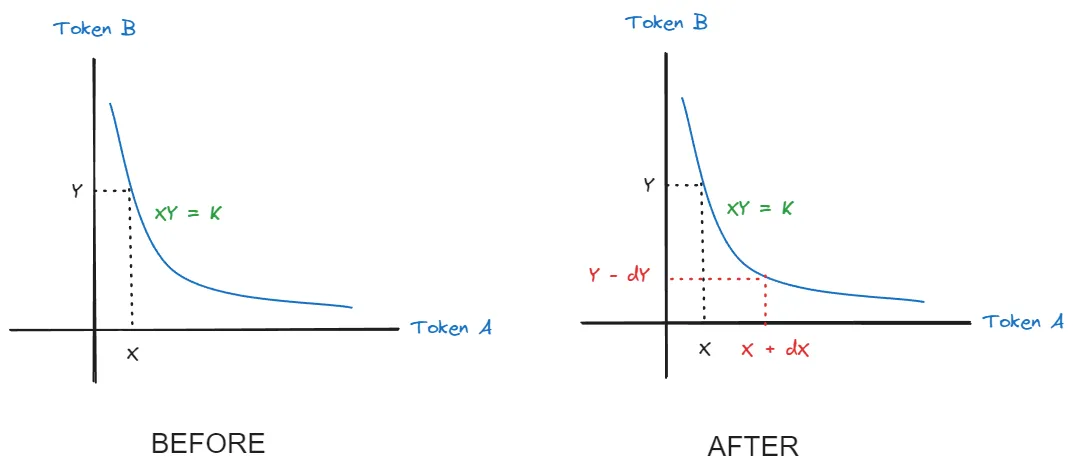
\includegraphics[width=1\textwidth]{figures/c1/AMM.png}
        \caption{Trạng thái của AMM trước và sau 1 lệnh bán dX.~\cite{AMM}}
        \label{fig:feature_interaction_example}
    \end{center}
\end{figure}
\hspace{-1cm}Từ đây, ta có công thức tính số lượng token nhận được
(\textbf{dY}) dựa vào số lượng token bán (\textbf{dX}) như sau:

\[XY = K \]
\[(X + dX)(Y - dY) = K \]
\[Y - dY = \frac{K}{X + dX} \]
\[dY = Y - \frac{XY}{X+dX} \]
\[dY = \frac{YX + YdX - XY}{X+dX}\]
\[dY = \frac{YdX}{X + dX}\quad \textbf{(2)} \]

\newpage

\hspace{-1cm}Như vậy, công thức (\textbf{2}) là công thức để tính lượng token
\textbf{dY} nhận được khi ta muốn trao đổi một lượng token \textbf{dX}

\subsection{Công thức tính lượng token share khi cung cấp thanh khoản}
\hspace{1cm}Khi một người dùng muốn đóng góp thanh khoản vào trong pool, giả sử
họ muốn thêm vào một lương là \textbf{dX} và \textbf{dY}. Lúc này, để duy trì
tỷ giá giữa hai token ở trong pool, ta có công thức ràng buộc giữa \textbf{dX}
và \textbf{dY} như sau:
\[XY = K \]
\[(X + dX)(Y + dY) = K' \]
\[\frac{X}{Y} = \frac{X + dX}{Y + dY} \]
\[{XdY} = {YdX} \]
\[\frac{X}{Y} = \frac{dX}{dY}\]
\[dY = \frac{YdX}{X}\quad \textbf{(3)} \]

\hspace{-1cm}Lúc này, AMM sẽ trả về cho người dùng một lượng token “share”. Khi
người dùng muốn rút thanh khoản ra khỏi pool, họ có thể sử dụng lượng token
“share” trước đó để thực hiện hành động này. Ta định nghĩa giá trị tổng thanh
khoản trong pool bằng một hàm như sau:

\[f(X,Y) = \sqrt(XY)\]
Với định nghĩa này, ta có:
\[L0 = f(X,Y)\]
\[L1 = f(X+dX, Y+dY)\]
Ta định nghĩa T là tổng lượng token “share” đã được tạo ra, s là lượng token
“share” mới sẽ được đúc cho người dùng. Lúc này, theo quy tắc tổng số lượng
token “share” sẽ tăng tỷ lệ thuận với sự gia tăng thanh khoản, ta có công thức
tính số lượng token “share” s như sau:

\[\frac{L1}{L0} = \frac{T + s}{T}\]
\[L1 * T = L0 * (T + s)\]
\[s = \frac{(L1 - L0) * T}{L0} \quad \textbf{(4)}\]
Như vậy (\textbf{4}) là công thức để tính lượng token “share” mà người dùng
nhận được khi cung cấp thanh khoản. Cuối cùng, ta sẽ xây dựng công thức khi
người dùng muốn sử dụng token “share” để rút thanh khoản ra khỏi pool.

\subsection{Công thức tính lượng token nhận được khi rút thanh khoản}
\hspace{1cm}Khi một người dùng muốn dừng cung cấp thanh khoản, họ sẽ trả vào
pool một lượng token “share” s. Như phần 1.5.2, ta định nghĩa T là tổng lượng
token “share” đã được tạo ra, giả sử dX và dY là lượng token mà người dùng này
nhận được sau khi ngừng cung cấp thanh khoản, ta có công thức tính dX và dY như
sau:

\[dX = \frac{s}{T} * X\]
\[dY = \frac{s}{T} * Y\]
Để chứng minh công thức trên, ta định nghĩa v là giá trị tổng thanh khoản được
rút ra, L là tổng giá trị thanh khoản ở trong pool, như vậy, ta có:

\[v = f(dX,dY) = \sqrt(dXdY)\]
\[L = f(X,Y) = \sqrt{XY}\]
Để duy trì tỷ lệ cân bằng giữa tổng giá trị thanh khoản và tổng lượng token
“share” được tạo ra, ta cần điều kiện như sau:

\[\frac{v}{L} = \frac{s}{T} \quad \textbf{(5)}\]
Để duy trì tỷ giá giữa hai token ở trong pool sau khi rút thanh khoản, ta đã
chứng minh ở mục 1.5.2 rằng  \[dY = \frac{Y}{X} * dX\]
Với công thức này, tiếp tục biến đổi điều kiện (\textbf{5}), ta có:
\[\frac{\sqrt{dXdY}}{\sqrt{XY}} = \frac{s}{T}\]
\[\frac{\sqrt{dX * \frac{Y}{X} * dX}}{\sqrt{XY}} = \frac{s}{T}\]
\[\frac{dX}{X} = \frac{s}{T}\]
\[dX = \frac{s}{T} * X \]
Như vậy, thông qua các mục vừa tìm hiểu, ta đã nắm được nguyên lý hoạt động cơ
bản của một AMM, các công thức trong trường hợp trao đổi token, thêm thanh
khoản và rút thanh khoản. Mô hình AMM sẽ được áp dụng xuyên suốt trong quá
trình mua/bán và trao đổi token trên hệ thống LaunchCrypt.

\section{Tổng quan về các thư viện và ngôn ngữ lập trình được sử dụng trong
  khóa luận}
\subsection{Ngôn ngữ lập trình Typescript, thư viện Reactjs và Nestjs}
\hspace{1cm}Trong quá trình phát triển LaunchCrypt, việc lựa chọn công nghệ phù
hợp đóng vai trò quan trọng trong việc đảm bảo hiệu suất, bảo mật và khả năng
mở rộng của dự án. Một trong những công nghệ chính được sử dụng là ngôn ngữ lập
trình TypeScript kết hợp với thư viện ReactJS cho phần frontend và NestJS cho
phần backend. Mỗi công nghệ này đều mang lại những lợi thế đáng kể, góp phần
đẩy nhanh quá trình phát triển sản phẩm và tạo nên một cấu trúc phần mềm vức
chắc.

TypeScript là một superset của JavaScript, bổ sung kiểu tĩnh và các tính năng
hướng đối tượng. Trong bối cảnh hệ thống của LaunchCrypt, Typescript thể hiện
khả năng hỗ trợ mạnh mẽ cho việc phát triển ứng dụng trên chuỗi khối khi các
chuỗi khối này
đều cung cấp SDK cho TypeScript, tạo điều kiện thuận lợi cho việc tương tác với
các mạng lưới như Avalanche, Solana, và Aptos. Ngoài ra, Typescript cũng giúp
lập trình viên phát hiện lỗi sớm trong quá trình phát triển, điều này là đặc
biệt quan trọng khi làm việc với các hợp đồng thông minh, khi các giao dịch
trên
chuỗi khối không có tính chất thu hồi.

\begin{figure}[H]
    \begin{center}
        \includegraphics[height=0.8\textwidth]{figures/c1/Blockchain
            Flow.drawio.png}
        \caption{Sử dụng Typescript SDK để tương tác với chuỗi khối.}
        \label{fig:feature_interaction_example}
    \end{center}
\end{figure}

Đối với phần frontend, ReactJS được chọn làm thư viện chính để xây dựng giao
diện người dùng. ReactJS, được phát triển bởi Facebook, là một trong những thư
viện JavaScript phổ biến nhất cho việc xây dựng giao diện người dùng động. Lý
do chính để chọn ReactJS cho LaunchCrypt bao gồm: Thứ nhất, hiệu suất cao của
ReactJS, nhờ vào cơ chế Virtual DOM, giúp tối ưu hóa việc render và cập nhật
UI, điều này rất quan trọng khi hiển thị dữ liệu thời gian thực như giá token
và trạng thái giao dịch. Thứ hai, cộng đồng lớn và hệ sinh thái phong phú của
ReactJS cung cấp nhiều thư viện và công cụ hỗ trợ, giúp đẩy nhanh quá trình
phát triển. Thứ ba, khả năng tái sử dụng component của ReactJS giúp tạo ra một
codebase dễ bảo trì và mở rộng. Cuối cùng, ReactJS kết hợp tốt với TypeScript,
cho phép xây dựng các components với kiểu dữ liệu rõ ràng, giảm thiểu lỗi và
cải thiện trải nghiệm phát triển.

Về phía backend, NestJS được lựa chọn làm thư viện chính. NestJS là một
framework Node.js tiến bộ, được phát triển từ ExpressJs và được xây dựng với
TypeScript. Có nhiều lý do khiến NestJS trở thành lựa chọn lý tưởng cho việc
xây dựng backend của LaunchCrypt: Đầu tiên, NestJS cung cấp một cấu trúc rõ
ràng và module hóa, điều này rất quan trọng khi xây dựng một ứng dụng phức tạp
như LaunchCrypt, giúp quản lý code dễ dàng hơn và cải thiện khả năng mở rộng.
Thứ hai, NestJS sử dụng Typescript, là một ngôn ngữ lập trình được hỗ trợ rất
tốt bởi những SDK được xây dựng sẵn trên các nền tảng chuỗi khối. Thứ ba,
NestJS cung
cấp nhiều decorators và utilities có sẵn, giúp đơn giản hóa việc xây dựng
RESTful APIs và WebSocket gateways, rất hữu ích cho việc xử lý các yêu cầu thời
gian thực trong ứng dụng DeFi. Cuối cùng, NestJS có khả năng tích hợp tốt với
nhiều thư viện và công cụ Node.js khác, cho phép linh hoạt trong việc lựa chọn
các công nghệ bổ sung cần thiết.
Việc kết hợp TypeScript, ReactJS và NestJS tạo nên một bộ công nghệ mạnh mẽ và
hiệu quả cho LaunchCrypt. TypeScript đảm bảo tính nhất quán và an toàn kiểu dữ
liệu xuyên suốt toàn bộ dự án. ReactJS cung cấp một nền tảng frontend linh hoạt
và hiệu suất cao, trong khi NestJS mang lại một backend có cấu trúc tốt và dễ
mở rộng. Việc lựa chọn ngôn ngữ lập trình cũng như các thư viện này giúp
LaunchCrypt bảo đảm được các tiêu chí về bảo mật và mở rộng, trong khi vẫn giữ
một cấu trúc phần mềm vững chắc và tốc độ phát triển nhanh.

\subsection{Ngôn ngữ lập trình Solidity, Rust và Move}
\hspace{1cm}Trong quá trình phát triển LaunchCrypt, một nền tảng đa chuỗi cho
việc tạo và giao dịch token, ba ngôn ngữ lập trình hợp đồng thông minh chính
được sử
dụng là Solidity, Rust và Move, mỗi ngôn ngữ đóng vai trò quan trọng trong việc
tương tác với các chuỗi khối khác nhau. Solidity, ngôn ngữ chủ đạo cho
Avalanche và nhiều chuỗi khối tương thích máy ảo Ethereum, được chọn vì khả
năng phát triển hợp đồng thông minh mạnh mẽ và hệ sinh thái rộng lớn, cho phép
LaunchCrypt tận dụng các thư viện có sẵn và công cụ phong phú trong lĩnh vực
DeFi. Rust, với hiệu suất cao và tính an toàn vượt trội, được sử dụng để phát
triển hợp đồng thông minh trên Solana, cung cấp khả năng xử lý giao dịch nhanh
chóng
và chi phí thấp, đặc biệt quan trọng cho các ứng dụng DeFi yêu cầu thông lượng
cao. Move, ngôn ngữ được thiết kế đặc biệt cho chuỗi khối Aptos, mang đến một
mô hình lập trình độc đáo tập trung vào bảo mật và linh hoạt trong quản lý tài
sản kỹ thuật số, giúp LaunchCrypt triển khai các tính năng cần thiết và đảm bảo
tính bảo mật trên các chuỗi khối mới nổi này. Quan trong hơn, các ngôn ngữ lập
trình này đã hỗ trợ các tiêu chuẩn token được định nghĩa trong mục 1.4, giúp
việc tạo và giao dịch token trở nên đơn giản và linh hoạt hơn. Việc kết hợp cả
ba ngôn ngữ này trong LaunchCrypt không chỉ cho phép dự án tận dụng ưu điểm
riêng của từng chuỗi khối, mà còn đảm bảo khả năng mở rộng trong tương lai, khi
các hệ sinh thái chuỗi khối tiếp tục phát triển và đa dạng hóa.

\section{Tổng kết chương}
Như vậy, qua chương đầu tiên, ta có thể nắm rõ được các khái niệm cơ bản về
công nghệ chuỗi khối và cơ chế hoạt động của nó, hiểu được bản chất của tài
chính phi tập
trung (DeFi) và vai trò của nó trong hệ sinh thái tài chính hiện đại. Chương
này cũng giới thiệu chi tiết về token, cấu trúc và đặc điểm của chúng trên các
chuỗi khối khác nhau, cũng như cơ chế hoạt động của thị trường tạo lập tự động
(AMM) - nền tảng cho các giao dịch trong DeFi. Bên cạnh đó, chương đầu tiên
cũng cung cấp tổng quan về các ngôn ngữ lập trình và thư viện quan trọng như
Solidity, Rust, Move, TypeScript, ReactJS và NestJS, tạo nền tảng vững chắc cho
việc phát triển dự án LaunchCrypt trong các chương tiếp theo.
